%%%%%%%%%%%%%%%%%%%%%%%%%%%%%%% beamer %%%%%%%%%%%%%%%%%%%%%%%%%%%%%%%%%%%%%%%%%%%%%%%%%
% To run - pdflatex filename.tex
%	   acroread filename.pdf
%%%%%%%%%%%%%%%%%%%%%%%%%%%%%%%%%%%%%%%%%%%%%%%%%%%%%%%%%%%%%%%%%%%%%%%%%%%%%%%%%%%%%%%%

\documentclass[compress,red,10pt]{beamer}
\mode<presentation>

\usetheme{Warsaw}
% other themes: AnnArbor, Antibes, Bergen, Berkeley, Berlin, Boadilla, boxes, CambridgeUS, Copenhagen, Darmstadt, default, Dresden, Frankfurt, Goettingen,
% Hannover, Ilmenau, JuanLesPins, Luebeck, Madrid, Maloe, Marburg, Montpellier, PaloAlto, Pittsburg, Rochester, Singapore, Szeged, classic

%\usecolortheme{lily}
% color themes: albatross, beaver, beetle, crane, default, dolphin, dov, fly, lily, orchid, rose, seagull, seahorse, sidebartab, structure, whale, wolverine

%\usefonttheme{serif}
% font themes: default, professionalfonts, serif, structurebold, structureitalicserif, structuresmallcapsserif

\hypersetup{pdfpagemode=FullScreen} % makes your presentation go automatically to full screen

% define your own colors:
\definecolor{Red}{rgb}{1,0,0}
\definecolor{Blue}{rgb}{0,0,1}
\definecolor{Green}{rgb}{0,1,0}
\definecolor{magenta}{rgb}{1,0,.6}
\definecolor{lightblue}{rgb}{0,.5,1}
\definecolor{lightpurple}{rgb}{.6,.4,1}
\definecolor{gold}{rgb}{.6,.5,0}
\definecolor{orange}{rgb}{1,0.4,0}
\definecolor{hotpink}{rgb}{1,0,0.5}
\definecolor{newcolor2}{rgb}{.5,.3,.5}
\definecolor{newcolor}{rgb}{0,.3,1}
\definecolor{newcolor3}{rgb}{1,0,.35}
\definecolor{darkgreen1}{rgb}{0, .35, 0}
\definecolor{darkgreen}{rgb}{0, .6, 0}
\definecolor{darkred}{rgb}{.75,0,0}

\xdefinecolor{olive}{cmyk}{0.64,0,0.95,0.4}
\xdefinecolor{purpleish}{cmyk}{0.75,0.75,0,0}

% can also choose different themes for the "inside" and "outside"

% \usepackage{beamerinnertheme_______}
% inner themes include circles, default, inmargin, rectangles, rounded

% \usepackage{beamerouterthemesmoothbars}
% outer themes include default, infolines, miniframes, shadow, sidebar, smoothbars, smoothtree, split, tree

\useoutertheme[subsection=false]{smoothbars}

% to have the same footer on all slides
%\setbeamertemplate{footline}[text line]{STUFF HERE!}
\setbeamertemplate{footline}[text line]{} % makes the footer EMPTY

% include packages
\usepackage{subfigure}
\usepackage{multicol}
\usepackage{amsmath}
\usepackage{epsfig}
\usepackage{graphicx}
\usepackage[all,knot]{xy}
\xyoption{arc}
\usepackage{url}
\usepackage{multimedia}
\usepackage{hyperref}
     
%%%%%%%%%%%%%%%%%%%%%%%%%%%%%%%%%%%%%%%%%%%%%%%%%%%%%%%%%%%%%%%%%%%%%%%%%%%%%%%%%%%%%%%%%%
%%%%%%%%%%%%%%%%%%%%%%%%%%%%%% Title Page Info %%%%%%%%%%%%%%%%%%%%%%%%%%%%%%%%%%%%%%%%%%%
%%%%%%%%%%%%%%%%%%%%%%%%%%%%%%%%%%%%%%%%%%%%%%%%%%%%%%%%%%%%%%%%%%%%%%%%%%%%%%%%%%%%%%%%%%

\title{Optimal Transport}
\subtitle{Preliminaries and Applications}
\author{Aidan Copinga}
\institute{Department of Mathematics\\ University of Utah}
\date{March 2022}

%%%%%%%%%%%%%%%%%%%%%%%%%%%%%%%%%%%%%%%%%%%%%%%%%%%%%%%%%%%%%%%%%%%%%%%%%%%%%%%%%%%%%%%%%%
%%%%%%%%%%%%%%%%%%%%%%%%%%%%%% Begin Your Document %%%%%%%%%%%%%%%%%%%%%%%%%%%%%%%%%%%%%%%
%%%%%%%%%%%%%%%%%%%%%%%%%%%%%%%%%%%%%%%%%%%%%%%%%%%%%%%%%%%%%%%%%%%%%%%%%%%%%%%%%%%%%%%%%%

\begin{document}

%%%%%%%%%%%%%%%%%%%%%%%%%%%%%%%%%%%%%%%%%%%%%%%%%%%%%%%%%%%%%%%%%%%%%%%%%%%%%%%%%%%%%%%%%%

\frame{
	\titlepage 
}

%%%%%%%%%%%%%%%%%%%%%%%%%%%%%%%%%%%%%%%%%%%%%%%%%%%%%%%%%%%%%%%%%%%%%%%%%%%%%%%%%%%%%%%%%%

%\section[Outline]{}	% this puts the outline before EACH section automatically & will highlight the section you're about to talk about
%\frame{\tableofcontents}

%%%%%%%%%%%%%%%%%%%%%%%%%%%%%%%%%%%%%%%%%%%%%%%%%%%%%%%%%%%%%%%%%%%%%%%%%%%%%%%%%%%%%%%%%%

\section{Introduction}
\subsection{The Problem}

%%%%%%%%%%%%%%%%%%%%%%%%%%%%%%%%%%%%%%%%%%%%%%%%%%%%%%%%%%%%%%%%%%%%%%%%%%%%%%%%%%%%%%%%%%

\frame{\frametitle{Optimal Transportation}
\begin{center}
\begin{block}<+->{History}
	\vspace{.1cm}
	Originally a question of optimally moving ammunition from factory to battlefield by Gaspard Monge in 1781 during Napoleonic France.
\end{block}
\vspace{0.5cm}
\begin{block}<+->{Formulation}
	\vspace{.1cm}
	Let $X$ and $Y$ be measure spaces with probability measures $\mu,\nu$ respectively. In order to transport $x\in X$ to $y\in Y$, we let $\mu(X) = \nu(Y)$. 
	The optimal transport problem is minimizing the total effort (through integrating over nonnegative $c: X\times Y\to \mathbb{R}$) over $\mu$ and $\nu$.
\end{block}
\end{center}
}
\frame{\frametitle{Optimal Transportation}
\begin{center}
\begin{figure}
	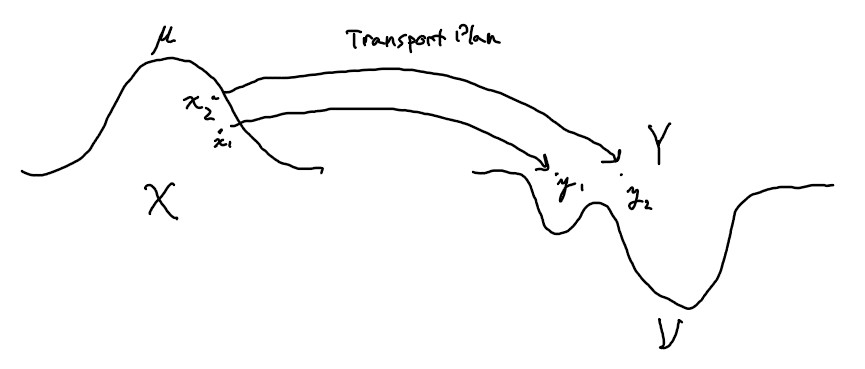
\includegraphics[scale=0.3]{transport.jpg}
	\caption{The question of optimal transport is how to move points of $X$ to $Y$.}
\end{figure}
\end{center}
}

%%%%%%%%%%%%%%%%%%%%%%%%%%%%%%%%%%%%%%%%%%%%%%%%%%%%%%%%%%%%%%%%%%%%%%%%%%%%%%%%%%%%%%%%%%
\frame{\frametitle{Monge Formulation}
\begin{center}
\begin{block}<+->{Transport Map}
	\vspace{.1cm}
	We call a function $T:X\to Y$ a \textit{transport map} if $T_\# \mu = \nu$ (that is, $T_\#\mu$ is the pushforward of $\nu$). Furthermore, we say $T$ transports $\mu$ to $\nu$.
\end{block}
\vspace{0.5cm}
\begin{block}<+->{Monge Formulation}
	\vspace{.1cm}
	Let
	\begin{equation}
		\mathcal{T}(\mu,\nu) = \left\{T: X\to Y \vert T_\#\mu = \nu,\,\,\text{$T$ measurable} \right\}
	\end{equation}
	Then we say that $\mathbb{M}(\mu,\nu)$ is the minimizer 
	\begin{equation}
		\mathbb{M}(\mu,\nu) = \inf_{T\in \mathcal{T}(\mu,\nu)} \int_{X}c(x,T(x))d\mu(x).
	\end{equation}
\end{block}
\end{center}
}
\frame{\frametitle{Monge Formulation Restrictions}
\begin{center}
\begin{block}<+->{Splitting Mass}
	\vspace{.1cm}
	Because we have $T: X\to Y$ with $T_\# \mu = \nu$, $T$ is bijective, so it cannot \textit{split mass}. This means for $y_1,y_2\in Y$, 
	a point $x\in X$ cannot have $T(x) = \{y_1,y_2\}$.
\end{block}
\begin{figure}
	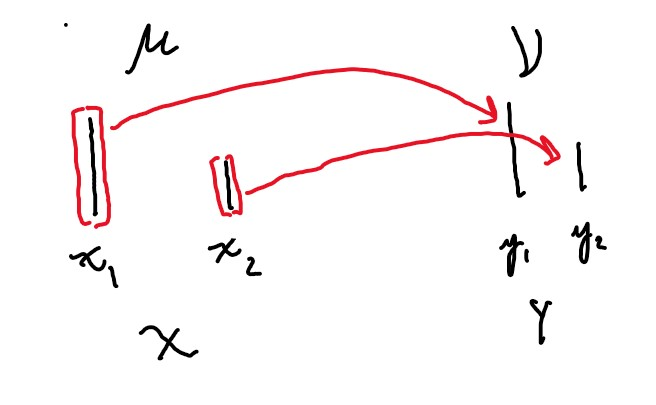
\includegraphics[scale=0.3]{monge.jpg}
	\caption{If we let $\mu = \frac{2}{3}\delta_{x_1} + \frac{1}{3}\delta_{x_2}$ and $\nu = \frac{2}{3}\delta_{y_1} + \frac{1}{3}\delta_{y_2}$ the only valid transport map is in red.}
\end{figure}
\end{center}
}
\frame{\frametitle{Kantorovich Formulation}
\begin{center}
\begin{block}<+->{Transport Plan}
	\vspace{.1cm}
	We call a measure $\pi\in \mathcal{P}(X\times Y)$ a \textit{transport plan} if for all measurable $A\subset X$ and $B\subset Y$,
	\begin{equation}\label{eqn:kant_constraints}
		\pi(A\times Y) = \mu(A)\quad \pi(X\times B) = \nu(B).
	\end{equation}
\end{block}
\begin{block}<+->{Kantorovich Formulation}
	\vspace{.1cm}
	Let
	\begin{equation}
		\Pi(\mu,\nu) = \left\{\pi \vert \pi\in\mathcal{P}(X\times Y)\text{ constrained by \eqref{eqn:kant_constraints}} \right\}
	\end{equation}
	Then we say that $\mathbb{K}(\mu,\nu)$ is the minimizer 
	\begin{equation}
		\mathbb{K}(\mu,\nu) = \inf_{\pi\in\Pi(\mu,\nu)} \int_{X\times Y}c(x,y)d\pi(x,y).
	\end{equation}
\end{block}
\end{center}
}
\frame{\frametitle{Kantorovich Formulation as a Relaxation}
\begin{center}
	We no longer have to be restricted to not splitting mass!
\begin{figure}
	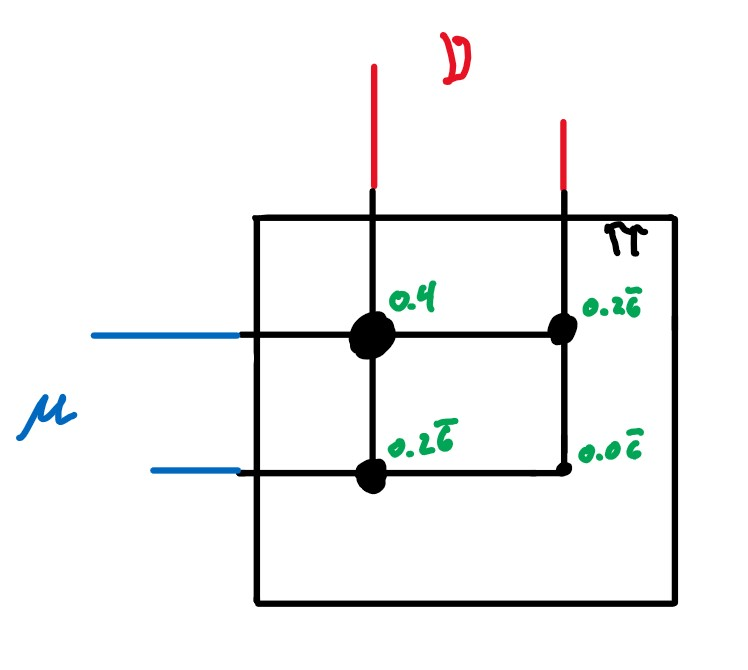
\includegraphics[scale=0.3]{discretekant.jpg}
	\caption{Using the same $\mu = \frac{2}{3}\delta_{x_1} + \frac{1}{3}\delta_{x_2}$ and $\nu = \frac{2}{3}\delta_{y_1} + \frac{1}{3}\delta_{y_2}$, we can define $\pi$ to no longer be diagonal (not surjective)}
\end{figure}
\end{center}
}
% \section{Duality}
% \frame{\frametitle{Shipper's Problem}
% It costs $c(x_1,y_1)$ dollars for a factory to transport coal from mine $x_1$ to factory $y_1$. I tell the mine owner that I can charge them $\phi(x_1)$ dollars to pick up at mine $x_1$ and charge $\psi(y_1)$ to deliver to factory $y_1$, then, in order for the factory owner to agree to my terms, 
% \[\phi(x)+\psi(y)\le c(x,y)\]
% for every mine $x$ and factory $y$. I can make this sum as close to $c(x,y)$ as I want, so I can maximize my profit while minimizing the factory owner's effort.
% }
% \frame{\frametitle{Shipper's Problem cont.}
% \begin{figure}
% 	\includegraphics[scale=0.3]{shippers.jpg}
% 	\caption{The owner has an easy option of just paying $c(M,F)$ for each mine and factory, or they can choose my strategy and pay me $\phi(M) + \psi(F)$.}
% \end{figure}
% }
% \frame{\frametitle{Deriving Duality}
% For a measure $\pi$, we see that we have $I[\pi, \phi,\psi]$ defined as
% \[\sup_{\phi\in C(X),\psi\in C(Y)} \left\{\int_X\phi(x)d\mu + \int_Y\psi(y)d\nu - \int_{X\times Y}(\phi(x)+\psi(y)d\pi)\right\}\]
% is $0$ when $\pi\in\Pi(\mu,\nu)$ and $+\infty$ otherwise. Now, writing this as a Kantorovich Problem for any positive radon measure $\pi$,
% \begin{equation}
% 	\mathbb{K}(\mu,\nu) = \inf_{\pi\ge 0}\left\{\int_{X\times Y} c(x,y)d\pi(x,y) + \sup_{\phi\in C(X),\psi\in C(Y)} I[\pi, \phi,\psi]\right\}
% \end{equation}
% We can informally$\star$ exchange the $\sup$ and $\inf$ to yield 
% \begin{equation}\label{eqn:minimax}
% 	\sup_{\phi,\psi}\left\{\int_X\phi(x)d\mu + \int_Y\psi(y)d\nu + \inf_{\pi\in\Pi}\int_{X\times Y}c(x,y) - (\phi(x)+\psi(y))d\pi\right\}
% \end{equation}
% }
% \frame{\frametitle{Kantorovich Duality}
% Following from \eqref{eqn:minimax}, we see that
% \[\inf_{\pi\in\Pi}\int_{X\times Y}c(x,y) - (\phi(x)+\psi(y))d\pi = \begin{cases}
% 	0 &\text{if $\phi(x)+\psi(y) \le c(x,y)$} \\
% 	+\infty &\text{otherwise.}
% \end{cases}\]
% This gives us the dual problem
% \begin{block}<+->{Dual Problem}
% 	\vspace{.1cm}
% 	For $\mu\in \mathcal{P}(X),\nu\in\mathcal{P}(Y)$ and a nonnegative cost function $c: X\times Y\to \mathbb{R}$,
% 	the Kantorovich dual problem is
% 	\begin{equation}
% 		\sup_{\phi\in C(X),\psi\in C(Y)}\left\{\int_X \phi(x)d\mu(x) + \int_Y\psi(Y)d\nu(y)\right\}
% 	\end{equation}
% 	subject to $\phi(x) + \psi(y) \le c(x,y)$.
% \end{block}
% }
% \frame{\frametitle{Discussing Informal Exchange}
% \begin{theorem}[Fenchel-Rockafeller Duality]
% Let $E$ be a normed vector space and $E^\star$ be its topological dual space. Let $\phi,\psi:E\to\mathbb{R}\cup\{+\infty\}$ be convex. If there is some $x_0\in E$ such that $\phi(x_0),\psi(x_0) <+\infty$ and $\phi$ is continuous at $x_0$, then
%   \begin{align*}
%     \inf_{x\in E}\{\phi(x)+\psi(x)\} = \sup_{f\in E^\star}\{-\phi^\star(-f)-\psi^\star(f)\}
%   \end{align*}
%   where   
%   \begin{equation}
%     \phi^\star(f) = \sup_{x\in E}\left[\langle f, x\rangle - \phi(x)\right].
%   \end{equation}  
%   is the Legendre-Fenchel Transform.
% \end{theorem}
% It's seen that this is a rigorous minimax theorem that justifies the exchange of the inf and sup.
% }
% \frame{\frametitle{Applications of Duality}
% Duality is important in showing the existence of transport maps, in fact,
% \begin{theorem}[Brenier Polar Factorization]
% 	Let $X,Y$ be measure spaces with probability measures $\mu,\nu$ respectively, then whenever $\mu$ does not give mass to small sets, there is a unique solution $\pi\in\Pi(\mu,\nu)$ to the Monge-Kantorovich problem with
% 	\[\pi = (\text{Id}\times \nabla \phi)_\# \mu\]
% 	where $\phi$ is a convex function defined $\mu$-almost everywhere. In other words, $\nabla \phi$ is a transport map.
% \end{theorem}
% The proof is quite rigorous involving Knott-Smith optimality, which uses Kantorovich Duality in its proof to describe the existence of a Kantorovich minimizer for lower-semicontinuous cost functions.
% }
\section{Wasserstein}
\frame{\frametitle{Wasserstein Distance}
Let's start by considering Kantorovich-Monge solutions to the transport problem with cost functions $c(x,y) = d(x,y)^p$ where $d$ is the distance on $X$ and $Y$.
Let $\Omega\subset X$ and set $x_0\in X$.
\[\mathcal{P}_p(X) = \left\{\mu\in\mathcal{P}(X):\int_{X}d(x,x_0)^p < +\infty\right\}\]
is the admissable class of measures $\mu$, even if $X$ is unbounded.
\begin{lemma}[Kantorovich-Monge forms a metric.]\label{lem:wass}
	Let $W_p(\mu,\nu) = \left[\inf_{\pi\in\Pi(\mu,\nu)}\int_{X\times X}d(x,y)^pd\pi(x,y)\right]^{1/p}$ defined for $\mu,\nu\in\mathcal{P}_P(X)$ be the Wasserstein Distance. This forms a metric on $X$.
\end{lemma}
}
\frame{\frametitle{Wasserstein Distance cont.}
We can informally interpret the Wasserstein Distance as the horizontal distance between measures.
\begin{figure}
	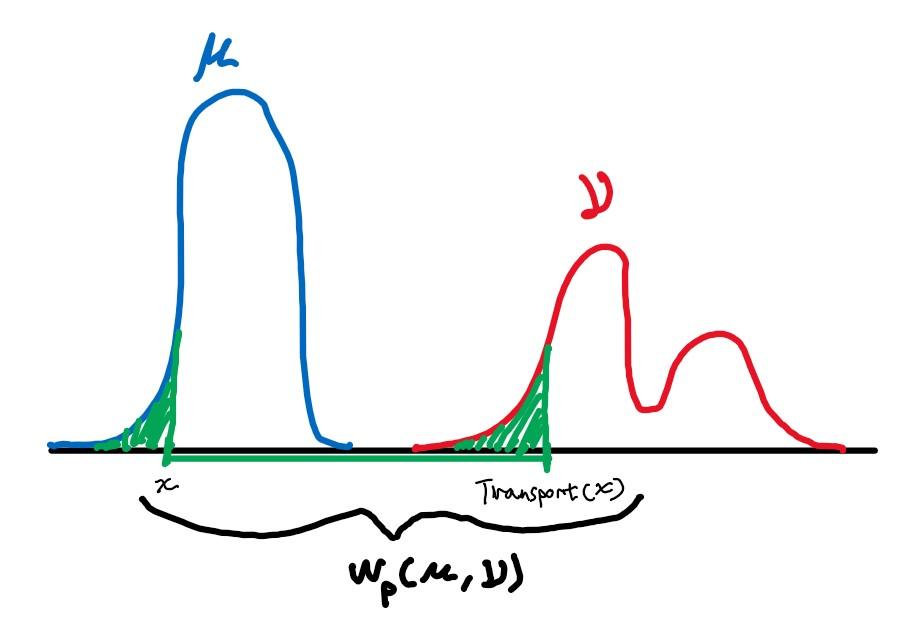
\includegraphics[scale=0.3]{wasserstein.jpg}
	\caption{The optimal transport (in green) between $\mu$ and $\nu$ describes the distance between points in $\mu$ and $\nu$ informally. Hence, this is the Wasserstein Distance.}
\end{figure}
}
% \frame{\frametitle{Wasserstein Distance Triangle Inequality}
% Assume $\mu,\nu,\eta\in \mathcal{P}_p(X)$ are absolutely continuous. Let $T$ be the optimal map from $\mu$ to $\eta$ and $S$ be the optimal map from $\eta$ to $\nu$.
% Then $S\circ T\in \mathcal{T}(\mu,\nu)$ because $(S\circ T)_\#\mu = S_\#(T_\#\mu) = S_\#\eta = \nu$. Hence,
% \begin{align*}
% 	W_p(\mu,\nu)) &\le \left(\int_Xd(x,(S\circ T)(x))^pd\mu(x)\right)^{1/p} = \|d(\text{Id},(S\circ T))\|_{L^p(\mu)} \\
% 	&\le \|d(\text{Id},T)\|_{L^p(\mu)} + \|d(T, S\circ T)\|_{L^p(\mu)} \\
% 	&= W_p(\mu,\eta) + \|d(\text{Id}, S)\|_{L^p(\eta)} \\
% 	&= W_p(\mu,\eta) + \int_{X}d(x,S(x))^pd\eta(x) = W_p(\mu,\eta) + W_p(\eta,\nu).
% \end{align*}
% }
% \frame{\frametitle{Proof of Lemma \ref{lem:wass}}
% I will just be doing the triangle inequality as it's the most involved.\newline
% Let $\lambda,\mu,\nu\in\mathcal{P}_p(X)$ with $\pi_1\in\Pi(\mu,\lambda)$ and $\pi_2\in\Pi(\lambda,\nu)$ be optimal in $W_p$. So there exists $\sigma\in \mathcal{P}(X^3)$ with
% 	\begin{equation}\label{eqn:gluing}
% 		(\gamma_{1,2})_\# \sigma = \pi_1,\quad (\gamma_{2,3})_\# \sigma = \pi_2,\text{ or } (\gamma_1)_\# \sigma = \mu, \quad (\gamma_3)_\#\sigma = \nu
% 	\end{equation}
% 	so we have $(\gamma_{1,3})_\#\sigma\in\Pi(\mu,\nu)$\footnote{This is the gluing lemma in Villani 7.6, I provide without proof, but his explanation is more detailed.}. 
% 	Now, using Minkowski's Inequality and \eqref{eqn:gluing},
% 	\begin{align*}
% 		W_p(\mu,\nu) &\le \left(\int_{X\times X}d(x,z)^p\gamma_{1,3}(x,z)\right)^{1/p} \\
% 		&\le \left(\int_{X^3}d(x,y)^p\sigma(x,y,z))\right)^{1/p}  +  \left(\int_{X^3}d(y,z)^p\sigma(x,y,z))\right)^{1/p} \\
% 		&= W_p(\mu,\lambda) + W_p(\lambda,\nu).
% 	\end{align*}
% }
% \frame{\frametitle{Wasserstein Topology}
% We see that if $x_n\to x$ in $X$ then
% \(W_p(\delta_{x_n},\delta_x) = d(x_n,x)^{\inf{(1,p)}} \to 0\). In general, this looks like
% \begin{theorem}[Wasserstein distances metrize weak convergence]
% 	Let $p\in(0,\infty)$, let $(\mu_k)_{k=1}^\infty$ be a sequence of measures in $\mathcal{P}_p(X)$ and $\mu\in \mathcal{P}(X)$, then the following are equivalent\footnote{Theorem 7.12 in Villani is much stronger and gives more equivalences, but due to time, I just want to make this statement.}:
% 	\begin{enumerate}[(i)]
% 		\item $W_p(\mu_k,\mu)\to 0$
% 		\item $\mu_k\to\mu$ in the weak sense, meaning for $h\in C_b(X)$,
% 		\[\lim_{k\to\infty}\int hd\mu_k = \int hd\mu.\]
% 	\end{enumerate} 
% \end{theorem}
% Furthermore, we usually look at $p=2$, and say $\mathbb{W}_2$ is the space $\mathcal{P}_2(X)$ endowed with the metric $W_2$.
% }
\section{Benamou-Brenier}
\frame{\frametitle{Continuity Equation}
The continuity equation is defined with 
\begin{equation}\label{eqn:continuity}p_t + \nabla \cdot (p\vec{v}) = 0\end{equation}
where $p$ is the fluid density and $\vec{v}$ is the flow vector field.\newline
Now, consider the smooth vector field $\vec{v}: [0,\infty)\times \mathbb{R}^n\to \mathbb{R}^n.$
Let $\phi_t: \mathbb{R}^n\to \mathbb{R}^n$ be the flow map such that for each $x\in \mathbb{R}^n$,
\[\partial_t\phi_t(x) = \vec{v}(t,\phi_t(x)),\quad \phi_0(x) = x.\]
Given some measure $p_0$ on $\mathbb{R}^n$, we can look at the family of measures 
\[p_t := (\phi_t)_\# p_0.\]
}
\frame{\frametitle{Benamou-Brenier}
Restrict $0\le t \le 1$ and fix source ($p_0$) and destination ($p_1$) densities.
\begin{theorem}[Benamou-Brenier]
	The minimum effort required to transport $p_0$ to $p_1$ by the flow of the vector field $\vec{v}$ with $p_t$,
	\begin{equation}
		\inf\left\{A[p_t,v]\bigg\vert\partial_t p_t + \nabla \cdot (p_t \vec{v}) = 0,p_t\vert_{t=0}=p_0, p_t\vert_{t=1}=p_1\right\}
	\end{equation} 
	is equivalent to the squared $2-$Wasserstein Distance $W_2(p_0,p_1)^2$ where \[A[p_t,v] = \int_0^1\int_{\mathbb{R}^n} |\vec{v}(t,x)|^2p_t(x)dxdt\]
\end{theorem}
$A$ is also called the action where the inner integral is the kinetic energy $E$ at time $t$. The action can also be interpreted as the average kinetic energy over $0\le t \le 1$. 
}
\frame{\frametitle{Applications}
Benamou-Brenier gives a hint to the Geodesic nature of the Wasserstein distance. That is, $p_t$ is a geodesic curve in $X$ between measures $p_0$ and $p_1$.\newline
Additionally, we can apply gradient flow structure onto the Wasserstein space with 
\[\partial_t\rho_t + \nabla\cdot(\vec{v}\rho_t) = 0.\]
}
\section{End}
\frame{\frametitle{Questions? Concerns?}
Recommended resources:
\begin{enumerate}
	\item Cedric Villani - Topics in Optimal Transportation (good overview)
	\item Fillipo Santambrogio - Optimal Transport for Applied Mathematicians (covers applications nicely)
	\item Luigi Ambrosio - Gradient Flows (this is dry and very technical)
	\item Matthew Thorpe - Introduction to Optimal Transport (nice summary of optimal transport, and covers geodesics in Wasserstein)
\end{enumerate}
This talk was meant to spur questions or ideas, and applications were covered without proof, so ask me through email at u0651651@utah.edu :)
}
%%%%%%%%%%%%%%%%%%%%%%%%%%%%%%%%%%%%%%%%%%%%%%%%%%%%%%%%%%%%%%%%%%%%%%%%%%%%%%%%%%%%%%%%%%
%%%%%%%%%%%%%%%%%%%%%%%%%%%%%% End Your Document %%%%%%%%%%%%%%%%%%%%%%%%%%%%%%%%%%%%%%%%%
%%%%%%%%%%%%%%%%%%%%%%%%%%%%%%%%%%%%%%%%%%%%%%%%%%%%%%%%%%%%%%%%%%%%%%%%%%%%%%%%%%%%%%%%%%

\end{document}

